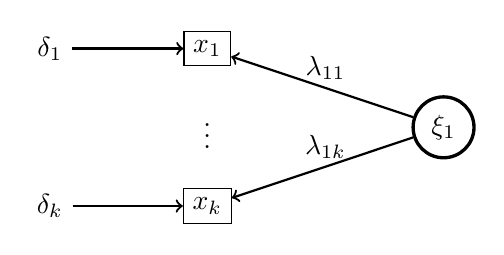
\begin{tikzpicture}[scale=1]
\tikzset{radial/.style={->,thick}}
\tikzstyle{item}=[draw,rectangle]
\tikzstyle{vl}=[draw,circle,very thick]
\node (d1)at(-2,11){$\delta_1$};
\node (d3)at(-2,9){$\delta_k$};
\node[item] (x1)at(0,11){$x_1$};
\node (x)at(0,10){$\vdots$};
\node[item] (x3)at(0,9){$x_k$};
\node (l1)at(1.5,10.75){$\lambda_{11}$};
\node (l3)at(1.5,9.75){$\lambda_{1k}$};
\node[vl] (vl1)at(3,10){$ \xi_1$};
\draw[radial] (vl1)--(x1);
\draw[radial] (vl1)--(x3);
\draw[radial] (d1)--(x1);
\draw[radial] (d3)--(x3);
\end{tikzpicture}
